\documentclass[a4paper,10pt]{article}
\usepackage[utf8]{inputenc}
\usepackage{graphicx}
\usepackage{tikz}
\usetikzlibrary{positioning}
\usepackage{listings}

\renewcommand\lstlistingname{Code Segment}

\definecolor{dkgreen}{rgb}{0,0.6,0}
\definecolor{gray}{rgb}{0.9,0.9,0.9}
\definecolor{mauve}{rgb}{1,0.4,0}

\lstset{frame=none,
  backgroundcolor=\color{gray},
  escapeinside={\%*}{*)},
  language=C++,
  aboveskip=3mm,
  belowskip=3mm,
  showstringspaces=false,
  columns=flexible,
  basicstyle={\small\ttfamily},
  numbers=left,
  numberstyle=\tiny\color{black},
  keywordstyle=\color{blue},
  commentstyle=\color{dkgreen},
  stringstyle=\color{mauve},
  breaklines=true,
  breakatwhitespace=true,
  tabsize=3,
  captionpos=b,
  xleftmargin=.25in,
  xrightmargin=.25in
}
\lstset{emph={
    signals,
    slots,
    Q_OBJECT
    },
    emphstyle={ \color{blue} }
}

%opening
\title{Ludo GUI}
\author{Nikolaj Iversen, Nicolai Lynnerup}

\begin{document}

\maketitle

\section{Getting the Game}
The game can be found at
\begin{verbatim}
https://gitlab.com/niive12/ludo-gui
\end{verbatim}
Or cloned with
\begin{verbatim}
git clone https://gitlab.com/niive12/ludo-gui.git
\end{verbatim}
The code depends on Qt and qmake.
\begin{verbatim}
mkdir -p ludo-gui/build
cd ludo-gui/build
qmake ../ludo
make
\end{verbatim}
And then the binary should be called \verb|ludo|.

\section{The Game Structure}
The ludo game is structured after a turn in the game.

Each turn is a series of communications between the game class and the player class.
In figure~\ref{fig:communications} the turn is illustrated.
The game class updates the GUI.
To make it easy to follow the game, two delays are inserted.
The speed of the game is currently set with the \verb|setGameDelay( msecs )| function in the main loop.
One is inserted just when the turn is given to a player and a longer one is given after the dice has been rolled.
The dice is printed in the GUI on a colored square, representing which player's turn it is to move.
In figure~\ref{fig:screenshot} the GUI can be seen.
The format of the positions is a \verb+std::vector<int>+.
In the beginning of the turn, both the positions and the dice roll are given to the player.
The two inputs are combined in a struct called \verb|positions_and_dice| which has the members \verb|pos| and \verb|dice|.

\begin{figure}
\centering
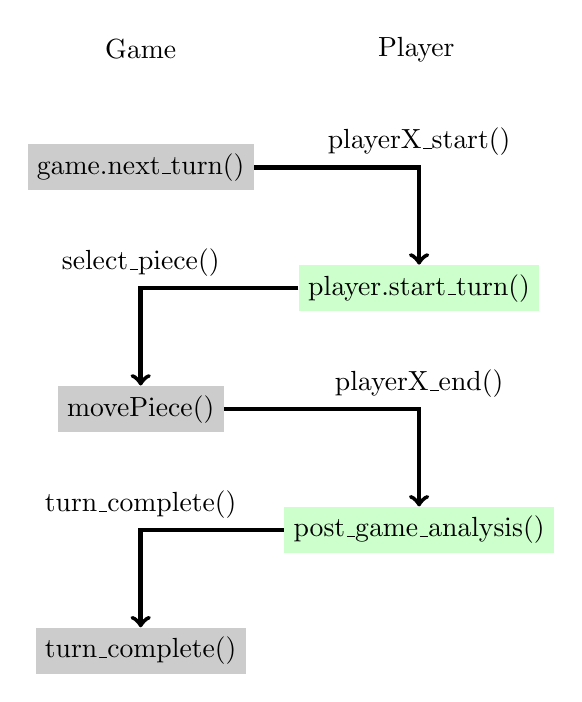
\begin{tikzpicture}[node distance = 5cm]
 \node[fill=black!20,name=NextT  ] at (0,0)                        {game.next\_turn()};
 \node[fill=green!20,name=StartT,below right of=NextT, yshift=2cm] {player.start\_turn()};
 \node[fill=black!20,name=MV,    below left of =StartT,yshift=2cm] {movePiece()};
 \node[fill=green!20,name=PGA,   below right of=MV,    yshift=2cm] {post\_game\_analysis()};
 \node[fill=black!20,name=TC,    below left of =PGA,   yshift=2cm] {turn\_complete()};
 \draw[->,ultra thick] (NextT)  -| (StartT)  node[midway,above]    {playerX\_start()};
 \draw[->,ultra thick] (StartT) -| (MV)      node[midway,above]    {select\_piece()};
 \draw[->,ultra thick] (MV)     -| (PGA)     node[midway,above]    {playerX\_end()};
 \draw[->,ultra thick] (PGA)    -| (TC)      node[midway,above]    {turn\_complete()};

 \node[above of=NextT,yshift=-3.5cm,name=title] {Game} node[right of=title, xshift=-1.5cm] {Player};
\end{tikzpicture}
\caption{A turn in the game.}\label{fig:communications}
\end{figure}

There is a lot of different rules to the game.
There is no special house rules added to the game.
The player has one chance to roll a 6 to get out.
A player only sends competitor home if they share the same end position.
This means if a piece is standing on every star, the first one will not be touched, but the second piece will be sent home.
Two pieces of the same team counts as a globe and will send the piece that moves to it home.

\begin{figure}
 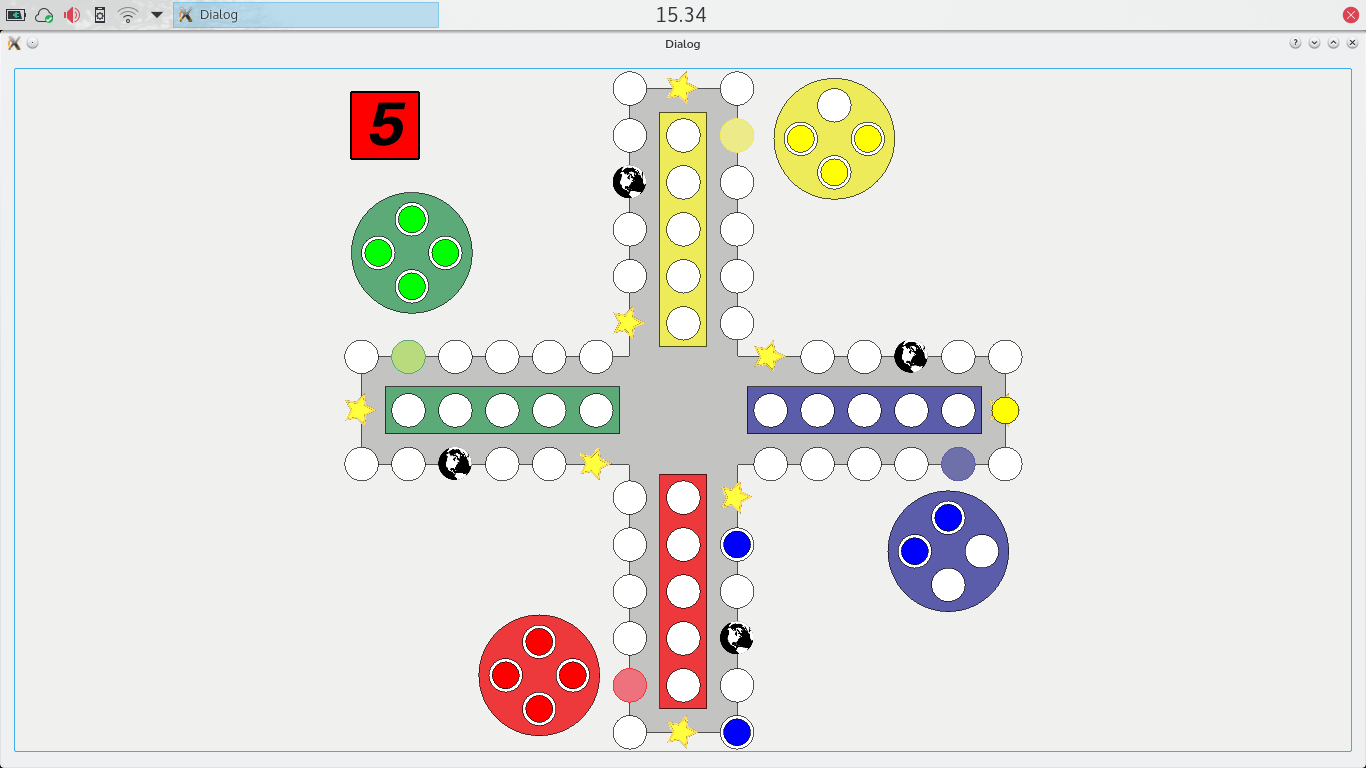
\includegraphics[width=\textwidth]{screenshot}
 \caption{Screenshot of the game.}
 \label{fig:screenshot}
\end{figure}

\section{Implementing a Player}
Two examples of a player is given in project.
They should be implemented as a class which has the signals described in the previous section.
For reference, it is also shown in \lstlistingname~\ref{ludo_player}.
The private values and variables are up to the programmer, but they are included for completeness.

The positions are always sorted, so that index 0-3 is the player's own pieces, 4-7 is the pieces of the next player clockwise on the board etc.
The positions are also moved, such that they are relative to the starting point of the player.
There are two ``off board'' positions a piece can be in.
It can be in the home position which is called -1, and it can be in goal position, called 99.
This allows for easy calculations of moving past field 57, so it moves backwards in the game.
Field 0 is the first globe outside the start position, colored like the home field.
Field 51 is the first step in the goal stretch.

An important note is that the player should check if it has won.
The \verb|turn_complete()| sends a bool to the game that, if true, will declare them the winner and stop the game, and should be false if they have not won the game.
The \verb|select_piece()| sends the index of the piece to the game.

\lstinputlisting[language=c++,
	firstnumber=7,
        firstline=7,
        lastline=22,
        caption={Class skeleton as found in Ludo/ludo\_player.h},
        label={ludo_player}
        ]{../ludo/ludo_player.h}

\end{document}
